\documentclass[a4paper]{article}
\usepackage[utf8]{inputenc}

\title{Plotting and fitting in Matlab}
\author{Joost Ouwerling}
\date{\today}

\usepackage{fullpage}
\usepackage{enumitem}
\usepackage{amsmath}
\usepackage{graphicx}
\usepackage{listings}
\usepackage{color}
\usepackage{placeins}
\usepackage{courier}
\usepackage{hyperref}

\definecolor{green}{rgb}{0,0.6,0}
\definecolor{gray}{rgb}{0.3,0.3,0.3}
\definecolor{mauve}{rgb}{0.58,0,0.82}

\lstdefinestyle{customc}{
  belowcaptionskip=1\baselineskip,
  breaklines=true,
  frame=L,
  xleftmargin=\parindent,
  language=matlab,
  numbers=left,
  showstringspaces=false,
  basicstyle=\ttfamily,
  keywordstyle=\bfseries\color{mauve},
  commentstyle=\ttfamily\color{green},
  identifierstyle=\color{black},
  stringstyle=\color{black},
}
\lstset{escapechar=@,style=customc}

\begin{document}

\maketitle

Most of you probably have encountered that Excel isn't the most friendly tool for plotting measurement data in a scientific accurate way and doing a proper linear fit (although it is certainly possible). This documents describes how to do it in Matlab, which is a useful skill to have during your studies. Matlab is installed in on the computers at the RUG campus and can also be accessed through uwp from home at \url{http://uwp.rug.nl/}. 


\section*{Code}

All necessary code is found in the listing below. You can type the commands after the \texttt{>>} signs in the command window.

You first define the x, y and y-errors in three vector variables. These have to be comma separated. Next, you plot an errorbar (see \url{http://www.mathworks.com/help/matlab/ref/errorbar.html} for an extensive explanation of this function) graph, which is essentially a scatterplot with vertical error bars. This function pops up a figure window. How to handle it is explained in the last section of this document. Next, you determine if you want to modify the range of the axis (could add some aesthetic improvements). 
\lstinputlisting[caption=Fitting in Matlab, style=customc]{plotfit.m}
\clearpage
The output of the linear fit function \texttt{fitlm} (see \url{http://www.mathworks.com/help/stats/fitlm.html}), for this data, is:
\begin{verbatim}
Linear regression model:
    y ~ 1 + x1

Estimated Coefficients:
                   Estimate       SE        tStat       pValue  
                   ________    ________    ________    _________

    (Intercept)    -0.15        0.17958    -0.83527      0.49145
    x1              1.07       0.065574      16.317    0.0037348


Number of observations: 4, Error degrees of freedom: 2
Root Mean Squared Error: 0.147
R-squared: 0.993,  Adjusted R-Squared 0.989
F-statistic vs. constant model: 266, p-value = 0.00373
\end{verbatim}
From this, all that is necessary is to see that the intercept is $-0.15 \pm 0.18$ and the linear parameter is $1.07 \pm 0.066$.

\section*{Adding a linear fit to the plot}
You can add a linear fit by clicking \texttt{Tools -> Basic Fitting} in the figure window, and selecting linear fit, as shown in the figure below. Via \texttt{Insert} you can add axis labels and a title to your graph. After you are happy with your plot, you can save it by \texttt{File -> Save As}.

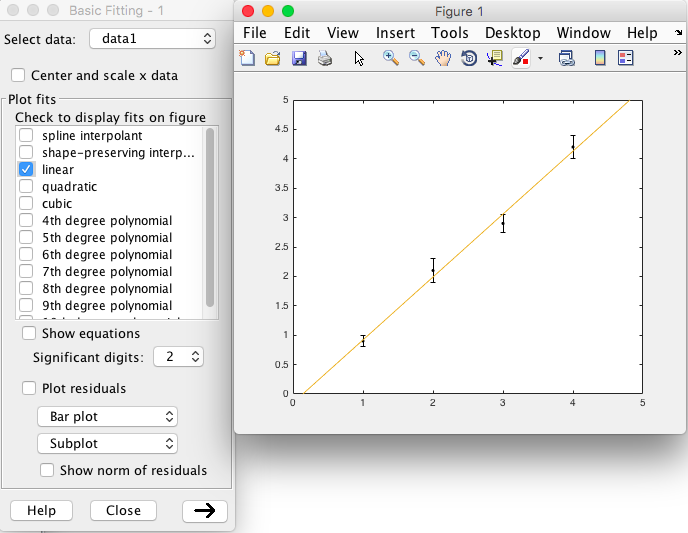
\includegraphics[width=\textwidth]{img.png}

\end{document}